\chapter{Исследовательская часть}

\section{Пример работы}

В листинге \ref{lst:ex} приведен пример работы программы. 
\begin{lstlisting}[label=lst:ex,caption=Функция нахождения расстояния Дамерау-Левенштейна нерекурсивным способом]
    ivanmamvriyskiy@MacBook-Pro-Ivan-2 main % go run main.go 
    Меню:
    1)Поиск дистанции;
    2)Проверка времени;
    3)Выход.
    Ввод: 
    1
    
    кабан
    бааан
    Матрица Левенштейна: 2
    Матрица Дамерау-Левенштейна: 2
    Рекурсивный алгоритм Дамерау-Левенштейна: 2
    Рекурсивный алгоритм Дамерау-Левенштейна с кэшем: 2
\end{lstlisting}

\section{Технические характеристики}

Технические характеристики устройства, на котором выполнялись замеры по времени, представлены далее:

\begin{itemize}
	\item Процессор --- 2 Гц 4‑ядерный процессор Intel Core i5;
	\item Оперативная память --- 16 ГБайт;
	\item Операционная система --- macOS Venura 13.5.2. 
\end{itemize}

\clearpage

\section{Время выполнения алгоритмов}

Результаты эксперимента замеров по времени приведены в таблице \ref{tab:perform}. В данной
таблице присутствуют поля с «-». Это обусловлено тем, что для 
рекурсивной реализации алгоритма достаточно приведенных замеров для 
построения графика. При длине строки большей 10 замер времени для рекурсивного
алгоритма будет долгим.
Замеры проводились на одинаковых длин строк от 1 до 10 вместе с рекурсивным, от 1 до 1000 без рекурсивного.

\begin{table}[!ht]
    \small
    \centering
    \caption{Замер времени работы алгоритмов в нс} 
    \label{tab:perform}
    \begin{tabular}{|r|r|r|r|r|r|}
    \hline
	Длина строк & Нерекурсив & Нерекурсив Д. Л. & Рекурсив с кэш. & Рекурсив \\ \hline
        1 & 600 & 500 & 500 & 0   \\ \hline
        2 & 700 & 500 & 600 & 1 000   \\ \hline
        3 & 700 & 700 & 2 600 & 2 000  \\ \hline
        4 & 1 000 & 900 & 1 500 & 6 000  \\ \hline
        5 & 1 100 & 600 & 1 100 & 20 000  \\ \hline
        6 & 1 200 & 1 400 & 3 200 & 124 000  \\ \hline
        7 & 1 600 & 1 900 & 3 500 & 568 000  \\ \hline
        8 & 1 600 & 3 300 & 3 700 & 2 881 000  \\ \hline
        9 & 1 700 & 4 400 & 2 900 & 13 157 000 \\ \hline
        10 & 2 300 & 4 100 & 3 100 & 44 023 000  \\ \hline
        100 & 61 400 & 101 100 & 193 400 & -  \\ \hline
        200 & 251 900 & 286 700 & 894 300 & -  \\ \hline
        300 & 497 800 & 572 900 & 223 3400 & -  \\ \hline
        400 & 904 100 & 1 165 600 & 44 19 400 & -   \\ \hline
        500 & 1 482 400 & 1 206 200 & 5 922 400 & -  \\ \hline
        600 & 1 669 200 & 1 896 700 & 9 061 400 & -  \\ \hline
        700 & 2 655 800 & 2 774 200 & 12 027 300 & -  \\ \hline
        800 & 3 376 800 & 3 298 500 & 17 409 200 & -  \\ \hline
        900 & 4 764 800 & 4 630 900 & 21 684 300 & -  \\ \hline
    \end{tabular}
\end{table}

% \begin{figure}[h]
% 	\centering
% 	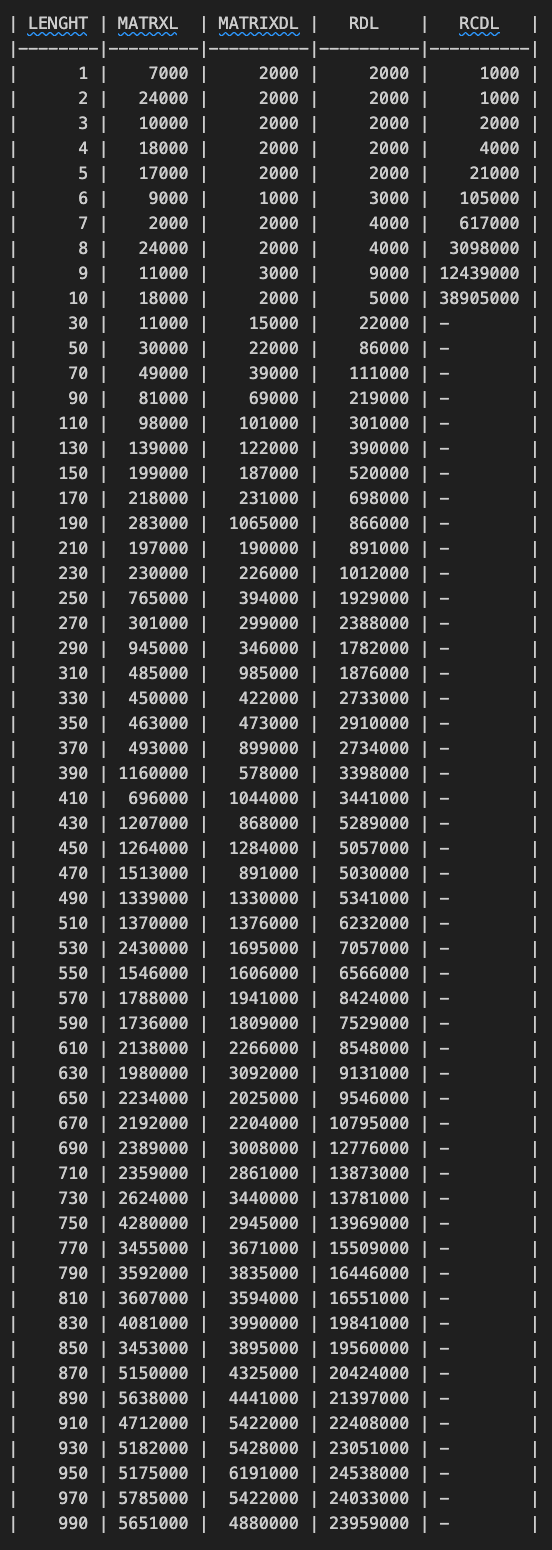
\includegraphics[width=0.85\textwidth]{img/resultTime.png}
% 	\caption{Демонстрация работы программы при поиске расстояний Левенштейна и Дамерау-Левенштейна}
% 	\label{img:demonstration}
% \end{figure}

На основе табличных данных построены графики \ref{img:demonstration} и
\ref{img:demonstr} зависимости времени 
выполнения алгоритма каждой из реализаций от длины строк. 

\begin{figure}[h]
	\centering
	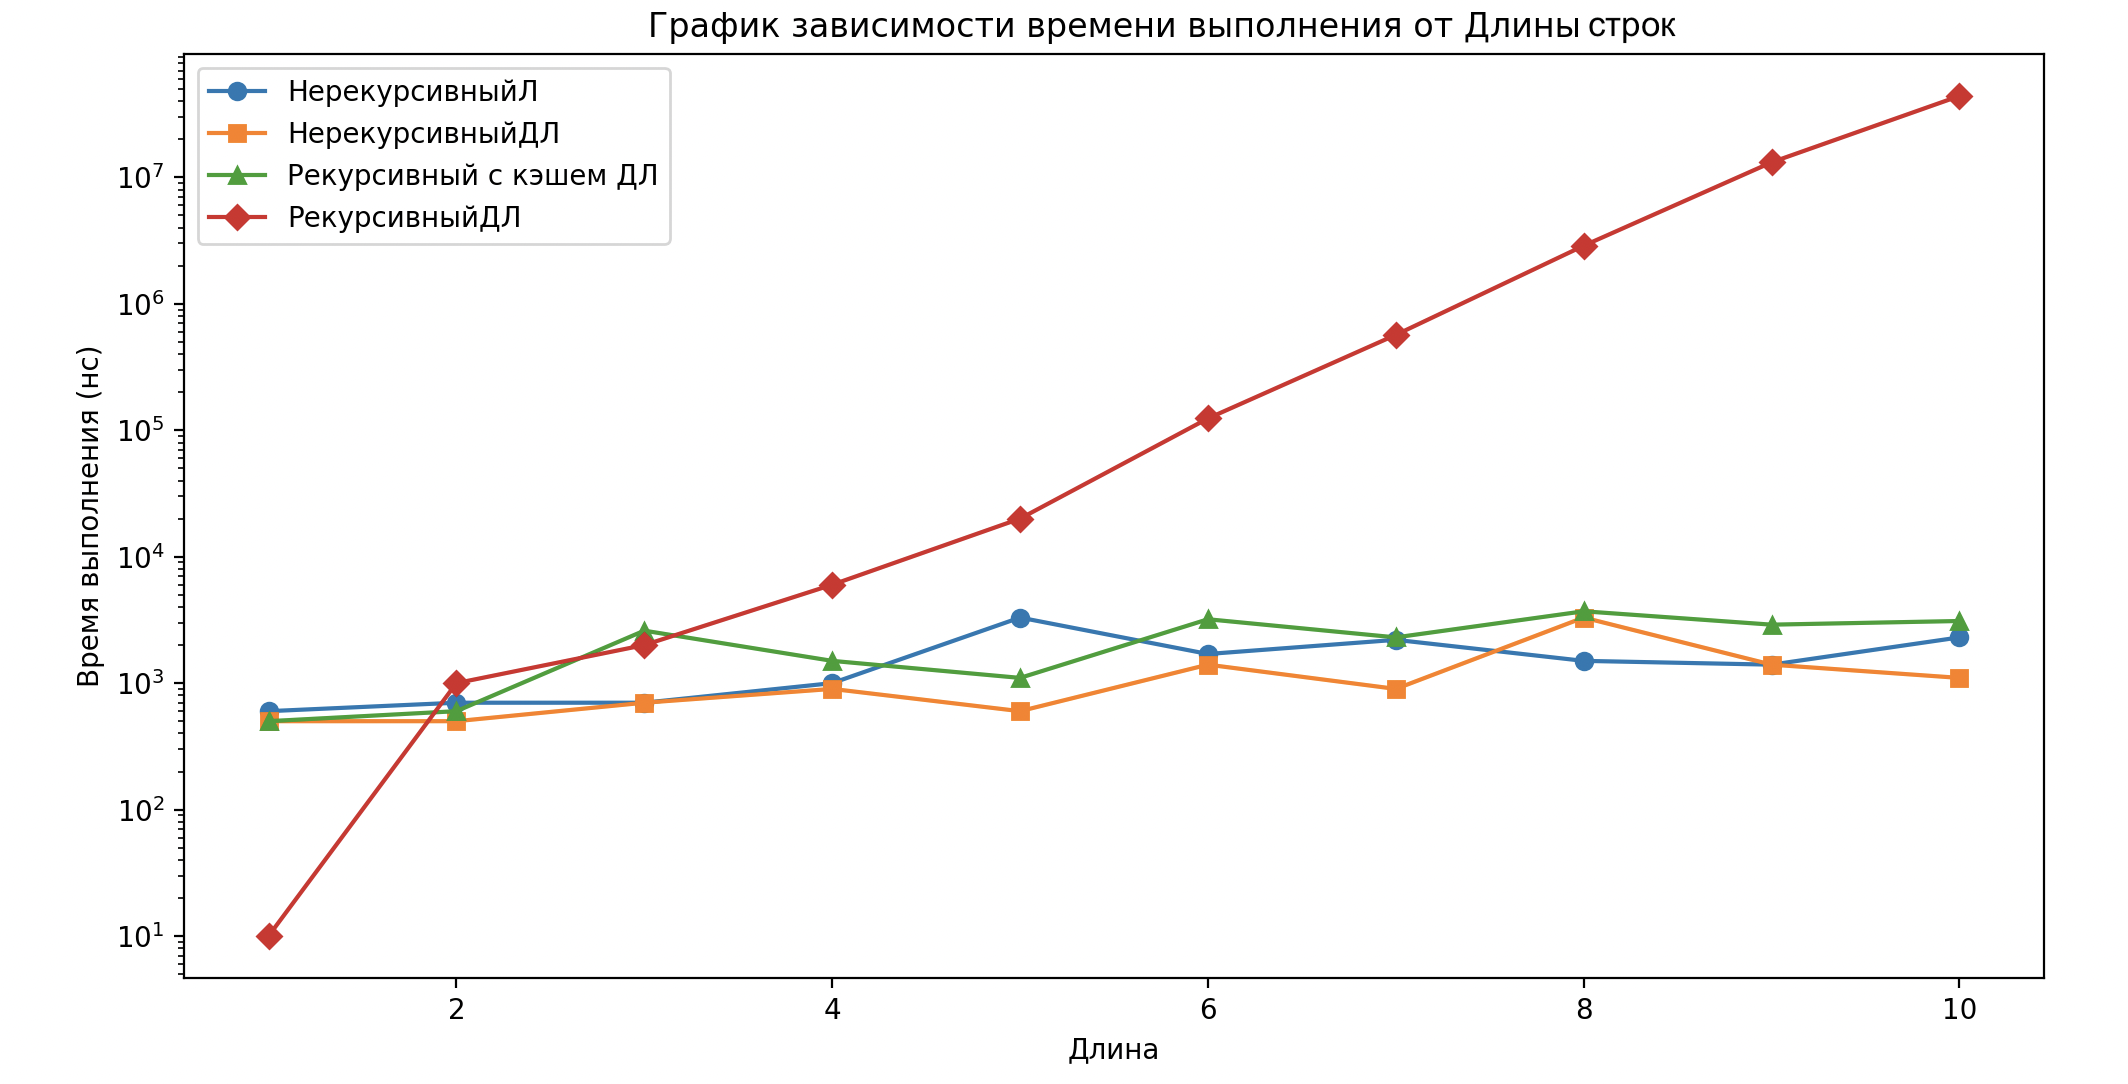
\includegraphics[width=1\textwidth]{img/graph15.png}
	\caption{График работы программы при поиске расстояний Левенштейна и Дамерау-Левенштейна}
	\label{img:demonstration}
\end{figure}

\begin{figure}[h]
	\centering
	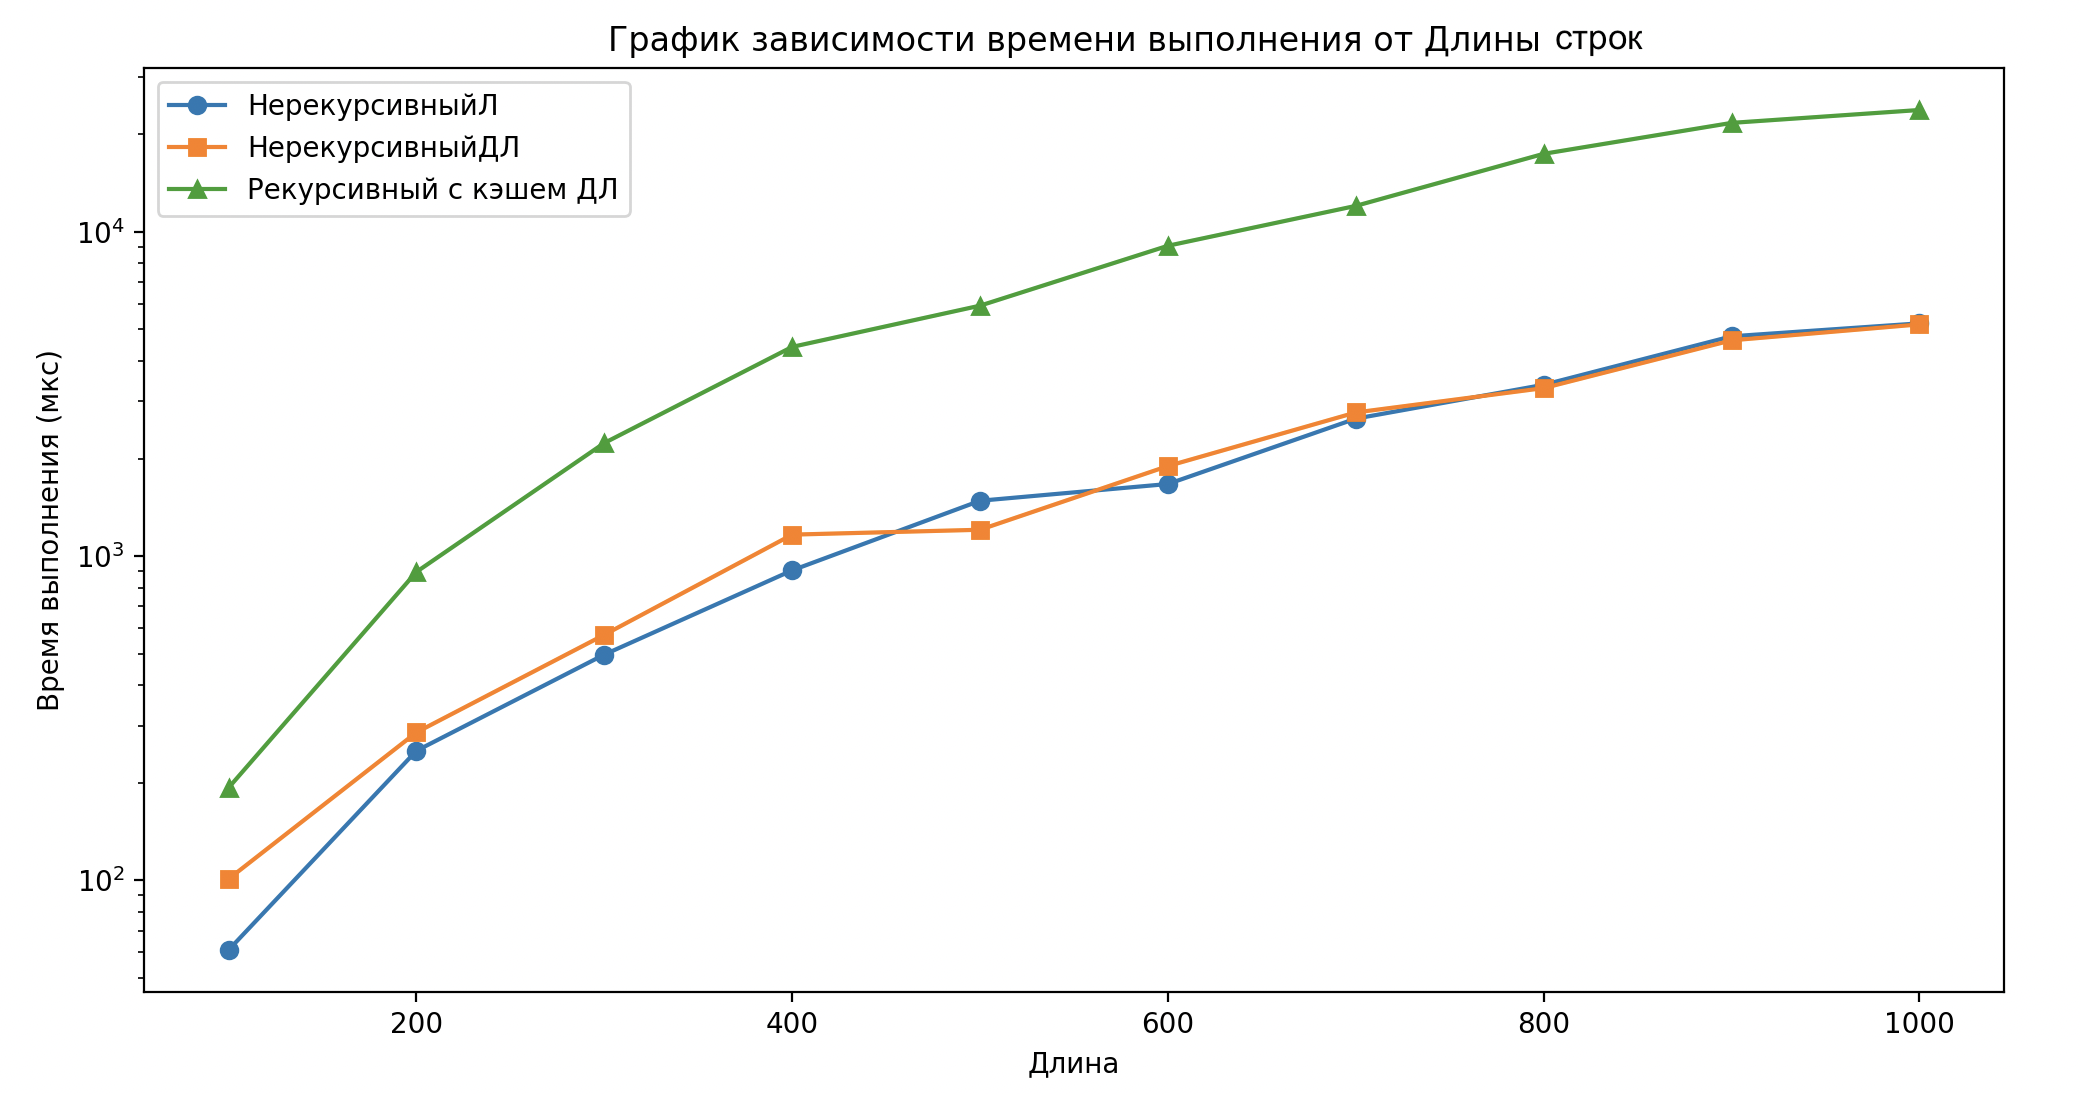
\includegraphics[width=1\textwidth]{img/allGraph.png}
	\caption{График работы программы при поиске расстояний Левенштейна и Дамерау-Левенштейна}
	\label{img:demonstr}
\end{figure}

\clearpage

Рекурсивный алгоритм поиска расстояния Левенштейна работает в 14 --- 40 
тысяч раз дольше алгоритмов, использующих матрицу, уже при значении 
длин строк, равных 10, что свидельствует о неэффективности этого алгоритма по времени. 
При длинах строк менее 200 символов разница по времени между 
итеративными реализациями и рекурсивной с кэшем незначительна, 
однако при увеличении 
длины строки алгоритм рекурсивного поиска расстояния Дамерау-Левенштейна с кэшем 
оказывается медленнее вплоть до 4 раз(при длинах строк от 700). 

Если рассматривать итерационные алгоритмы, то алгоритм Левенштейна работает немного быстрее,
чем алгоритм Дамерау-Левенштейна, так как во втором есть дополнительная проверка.

\clearpage

\section{Использование памяти}

Введем следующие обозначения:
\begin{itemize}
	\item$n$ --- длина строки $S_{1}$;
	\item$m$ --- длина строки $S_{2}$;
	\item$size()$ --- функция вычисляющая размер в байтах;
	\item $string$ --- строковый тип;
	\item $int$ --- целочисленный тип;
	\item $size\_t$ --- беззнаковый целочисленный тип.
\end{itemize}

Максимальная глубина стека вызовов при рекурсивной реализации нахождения расстояния Дамерау-Левенштейна равна сумме входящих строк, а на каждый вызов требуется 2 дополнительные переменные, соответственно, максимальный расход памяти равен:
\begin{equation}
	\label{eq:dl_rec_memory}
	(n + m) \cdot (2 \cdot size(string) + 3 \cdot size(int) + 2 \cdot sizeof(size\_t)),
\end{equation}
где:
\begin{itemize}
	\item $2 \cdot size(string)$ --- хранение двух строк;
	\item $2 \cdot size(size\_t)$ --- хранение размеров строк;
	\item $2 \cdot size(int)$ --- дополнительные переменные;
	\item $size(int)$ --- адрес возврата.
\end{itemize}

Для рекурсивного алгоритма c кэшированием поиска расстояния Дамерау-Левенштейна будет теоретически схож с расчетом в формуле (\ref{eq:dl_rec_memory}), но также учитывается матрица, соответственно, максимальный расход памяти равен:
\begin{equation}
	\label{eq:dl_hash_memory}
	\begin{aligned}
		(n + m) \cdot (2 \cdot size(string) + 3 \cdot size(int) + 2 \cdot size(size\_t)) + \\
		+ (n + 1) \cdot (m + 1) \cdot size(int)
	\end{aligned}
\end{equation}
Использование памяти при итеративной реализации алгоритма поиска расстояния Левенштейна теоретически равно:
\begin{equation}
	\label{eq:lev_mtr_memory}
	\begin{aligned}
		(n + 1) \cdot (m + 1) \cdot size(int) + 2 \cdot size(string) + 2 \cdot size(size\_t) + \\
		+ size(int **) + (n + 1) \cdot size(int *) + 2 \cdot size(int),
	\end{aligned}
\end{equation}
где 
\begin{itemize}
	\item $2 \cdot size(string)$ --- хранение двух строк;
	\item $2 \cdot size(size\_t)$ --- хранение размеров матрицы;
	\item $(n + 1) \cdot (m + 1) \cdot size(int)$ --- хранение матрицы;
	\item $size(int **) + (n + 1) \cdot size(int *)$ --- указатель на матрицу;
	\item $size(int)$ --- дополнительная переменная для хранения результата;
	\item $size(int)$ --- адрес возврата.
\end{itemize}

Использование памяти при итеративной реализации алгоритма поиска расстояния Дамерау-Левенштейна теоретически равно:
\begin{equation}
	\label{eq:dl_mtr_memory}
	\begin{aligned}
		(n + 1) \cdot (m + 1) \cdot size(int) + 2 \cdot size(string) + 2 \cdot size(size\_t) + \\
		+ size(int **) + (n + 1) \cdot size(int *) + 3 \cdot size(int),
	\end{aligned}
\end{equation}
где 
\begin{itemize}
	\item $2 * size(string)$ --- хранение двух строк;
	\item $2 \cdot size(size\_t)$ --- хранение размеров матрицы;
	\item $(n + 1) \cdot (m + 1) \cdot size(int)$ --- хранение матрицы;
	\item $size(int **) + (n + 1) \cdot size(int *)$ --- указатель на матрицу;
	\item $2 \cdot size(int)$ --- дополнительные переменные;
	\item $size(int)$ --- адрес возврата.
\end{itemize}

В таблице \ref{tab:tabM} представлены замеры памяти при работе данных алгоритмов в зависимости
от длины строк.

\begin{table}[!ht]
    \small
    \centering
    \caption{\label{tab:tabM} Количество используемой памяти при работе данных алгоритмов
    в зависимости от длины строк.}
    \begin{tabular}{|r|r|r|r|r|r|}
    \hline
        Длина строк & Нерекурсив Л & Нерекурсив ДЛ & Рекурсив кэш & Рекурсив\\ \hline
        1 & 120 & 128 & 200 & 144  \\ \hline
        2 & 168 & 176 & 392 & 288  \\ \hline
        3 & 232 & 240 & 600 & 432  \\ \hline
        4 & 312 & 320 & 824 & 576  \\ \hline
        5 & 408 & 416 & 1 064 & 720  \\ \hline
        6 & 520 & 528 & 1 320 & 864  \\ \hline
        7 & 648 & 656 & 1 592 & 1 008  \\ \hline
        8 & 792 & 800 & 1 880 & 1 152  \\ \hline
        9 & 952 & 960 & 2 184 & 1 296  \\ \hline
        10 & 1 128 & 1 136 & 2 504 & 1 440  \\ \hline
        100 & 82 488 & 82 496 & 96 824 & 14 400  \\ \hline
        200 & 324 888 & 324 896 & 353 624 & 28 800  \\ \hline
        300 & 727 288 & 727 296 & 770 424 & 43 200  \\ \hline
        400 & 1 289 688 & 1 289 696 & 1 347 224 & 57 600  \\ \hline
        500 & 2 012 088 & 2 012 096 & 2 084 024 & 72 000  \\ \hline
        600 & 2 894 488 & 2 894 496 & 2 980 824 & 86 400  \\ \hline
        700 & 3 936 888 & 3 936 896 & 4 037 624 & 100 800  \\ \hline
        800 & 5 139 288 & 5 139 296 & 5 254 424 & 115 200  \\ \hline
        900 & 6 501 688 & 6 501 696 & 6 631 224 & 129 600  \\ \hline
        1000 & 8 024 088 & 8 024 096 & 8 168 024 & 144 000 \\ \hline
    \end{tabular}
\end{table}

\section{Вывод}

В данном разделе было произведено сравнение количества затраченного времени 
и памяти алгоритмов поиска расстояний Левенштейна и Дамерау-Левенштейна. 
Наименее затратным по времени оказался рекурсивный алгоритм нахождения расстояния 
Дамерау-Левенштейна.

Приведенные характеристики показывают, что рекурсивная реализация алгоритма 
во много раз проигрывает по времени. В связи с этим, рекурсивные алгоритмы следует 
использовать лишь для малых размерностей строк (<= 10 символов).

Так как во время печати очень часто возникают ошибки связанные с 
транспозицией букв, алгоритм нерекурсивного поиска расстояния Дамерау-Левенштейна 
является наиболее предпочтительным, не смотря на то, что он незначительно 
проигрывает по времени и памяти алгоритму Левенштейна.

Самым затрачиваемым по памяти алгоритмом получился рекурсивный алгоритм Дамерау-Левенштейна с кэшем.
Итеративные алгоритмы проигрывают рекурсивному алгоритму по расходу памяти.


